\documentclass[../MasterThesis.tex]{subfiles}
\graphicspath{ {./assets/images/} }


%----------------------------------------------------------------------------
%----------------------------------------------------------------------------

\begin{document}
	
	
%
%
%
%
%=======================================================================================================
%
%
%
%
%=======================================================================================================
% CHAPTER: CONCLUSION AND FUTURE WORK
%=======================================================================================================
\newpage
\section{Conclusion} \label{section:conclusion}


%-------------------------------------------------------------------------------------------------------
\subsection{Summary} \label{subsection:summary}
% Summarize the key findings and outcomes of the research.


%-------------------------------------------------------------------------------------------------------
\subsection{Contributions and Limitations} \label{subsection:contributionsandlimitations}
% Highlight your contributions to the field.
% Discuss any limitations encountered during the research.


%-------------------------------------------------------------------------------------------------------
\subsection{Future Work} \label{subsection:futurework}
% Suggest possible extensions or improvements to your work.

\subsubsection*{Video Presets}

Video presets, also known as video filters or video effects, are pre-configured settings or adjustments that can be applied to videos to achieve specific visual styles or effects. 
These presets often include templates for colour grading. 
Video presets are commonly used in video editing software and social media platforms. They provide the user with options to customize their videos easily. 

One example for video presets can be seen in Figure~\ref{figure:app}, where the presets in Adobe Premiere Pro with the \textit{Magic Bullet Looks} plug-in are shown.~\cite{premierepro, magicbullet}

\begin{figure}[H]
	
	\centering
	
	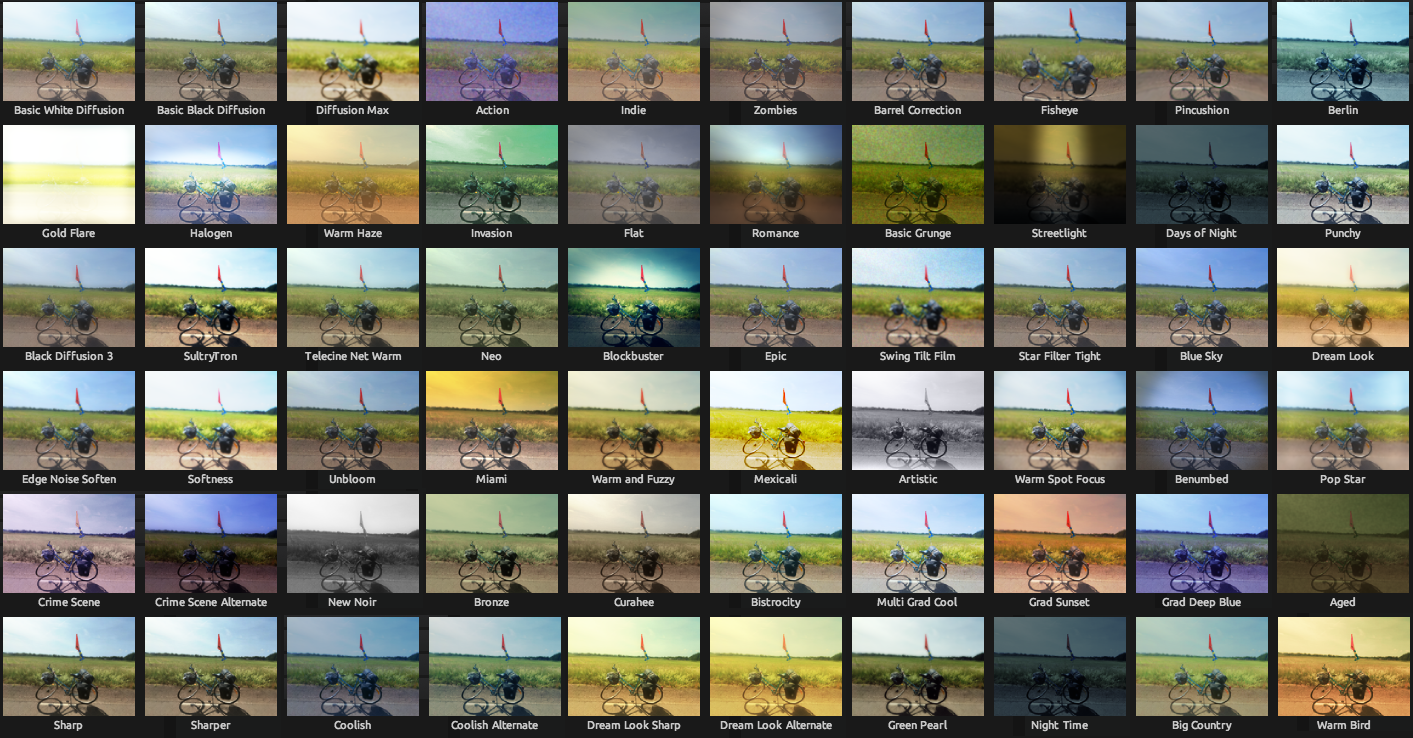
\includegraphics[width=0.99\textwidth]{app.png}
	
	\caption[Presets in Adobe Premiere Pro (\textit{Magic Bullet Looks})]{Presets in Adobe Premiere Pro with the plug-in \textit{Magic Bullet Looks}~\cite{premierepro, magicbullet}}
	\label{figure:app}
	
\end{figure}

Implementing options for the application of those presets is an interesting opportunity for future work. To implement this, different Melt filters can be used or combined. Different options for those Melt filters can be seen in Appendix~\ref{appendix:differentMeltFilter}.




	
	
	
\end{document}